\begin{center}

\includegraphics[width=0.8\textwidth]{content/3/chapter6/images/28.png}\\
Cippi sings in the choir
\end{center}


\begin{tcolorbox}[breakable,enhanced jigsaw,colback=blue!5!white,colframe=blue!75!black,title={Compiler Support for Synchronized Output Streams}]
	
At the end of 2020, only GCC 11 supports synchronized output streams.
	
\end{tcolorbox}

What happens when you write without synchronization to std::cout?

\hspace*{\fill} \\ %插入空行
\noindent
Non-synchronized access to std::cout
\begin{lstlisting}[style=styleCXX]
// coutUnsynchronized.cpp

#include <chrono>
#include <iostream>
#include <thread>

class Worker{
public:
	Worker(std::string n):name(n) {};
	void operator() (){
		for (int i = 1; i <= 3; ++i) {
			// begin work
			std::this_thread::sleep_for(std::chrono::milliseconds(200));
			// end work
			std::cout << name << ": " << "Work " << i << " done !!!" << '\n';
		}
	}
private:
	std::string name;
};


int main() {

	std::cout << '\n';
	
	std::cout << "Boss: Let's start working.\n\n";
	
	std::thread herb= std::thread(Worker("Herb"));
	std::thread andrei= std::thread(Worker(" Andrei"));
	std::thread scott= std::thread(Worker(" Scott"));
	std::thread bjarne= std::thread(Worker(" Bjarne"));
	std::thread bart= std::thread(Worker(" Bart"));
	std::thread jenne= std::thread(Worker(" Jenne"));
	
	
	herb.join();
	andrei.join();
	scott.join();
	bjarne.join();
	bart.join();
	jenne.join();
	
	std::cout << "\n" << "Boss: Let's go home." << '\n';
	
	std::cout << '\n';

}
\end{lstlisting}

The boss has six workers (lines 29 - 34). Each worker has to take care of three work packages that take 1/5 second each (line 13). After the worker is done with his work package, he screams out loudly to the boss (line 15). Once the boss receives notifications from all workers, he sends them home (line 44).

What a mess for such a simple workflow! Each worker screams out his message ignoring his coworkers!

\begin{center}
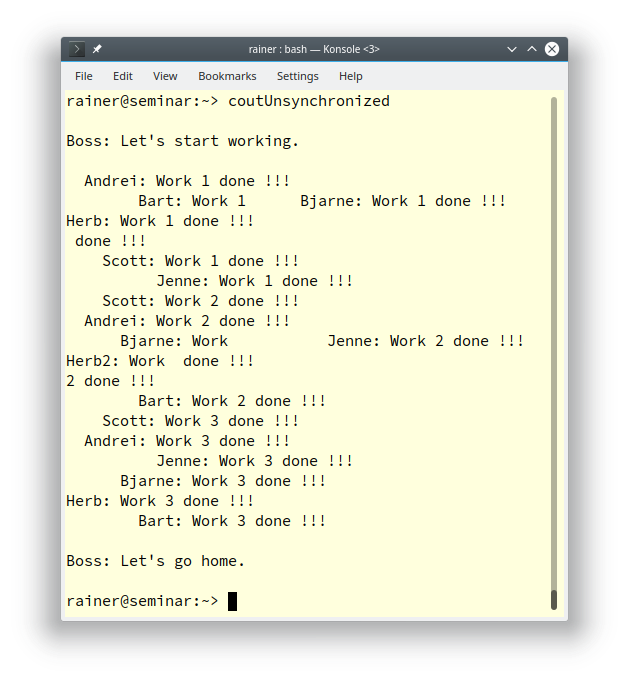
\includegraphics[width=0.8\textwidth]{content/3/chapter6/images/29.png}\\
Non-synchronized writing to std::cout
\end{center}

\begin{tcolorbox}[breakable,enhanced jigsaw,colback=blue!5!white,colframe=blue!75!black,title={std::cout is thread-safe}]
	
The C++11 standard guarantees that you need not protect std::cout. Each character is written atomically. More output statements like those in the example may interleave. This interleaving is only a visual issue; the program is well-defined. This remark is valid for all global stream objects. Insertion to and extraction from global stream objects (std::cout, std::cin, std::cerr, and std::clog) is thread-safe. To put it more formally: writing to std::cout is not participating in a data race, but does create a race condition. This means that the output depends on the interleaving of threads.
	
\end{tcolorbox}

How can we solve this issue? With C++11, the answer is straightforward: use a lock such as \href{https://en.cppreference.com/w/cpp/thread/lock_guard}{lock\_guard} to synchronize the access to std::cout.

\hspace*{\fill} \\ %插入空行
\noindent
Synchronized access to std::cout
\begin{lstlisting}[style=styleCXX]
// coutSynchronized.cpp

#include <chrono>
#include <iostream>
#include <mutex>
#include <thread>

std::mutex coutMutex;

class Worker{
public:
	Worker(std::string n):name(n) {};
	
	void operator() () {
		for (int i = 1; i <= 3; ++i) {
			// begin work
			std::this_thread::sleep_for(std::chrono::milliseconds(200));
			// end work
			std::lock_guard<std::mutex> coutLock(coutMutex);
			std::cout << name << ": " << "Work " << i << " done !!!\n";
		}
	}
private:
	std::string name;
};


int main() {

	std::cout << '\n';
	
	std::cout << "Boss: Let's start working." << "\n\n";
	
	std::thread herb= std::thread(Worker("Herb"));
	std::thread andrei= std::thread(Worker(" Andrei"));
	std::thread scott= std::thread(Worker(" Scott"));
	std::thread bjarne= std::thread(Worker(" Bjarne"));
	std::thread bart= std::thread(Worker(" Bart"));
	std::thread jenne= std::thread(Worker(" Jenne"));
	
	herb.join();
	andrei.join();
	scott.join();
	bjarne.join();
	bart.join();
	jenne.join();
	
	std::cout << "\n" << "Boss: Let's go home." << '\n';
	
	std::cout << '\n';

}
\end{lstlisting}

The coutMutex in line 8 protects the shared object std::cout. Putting the coutMutex into a std::lock\_guard guarantees that the coutMutex is locked in the constructor (line 19) and unlocked in the destructor (line 21) of the std::lock\_guard. Thanks to the coutMutex guarded by the coutLock the mess becomes a harmony.

\begin{center}
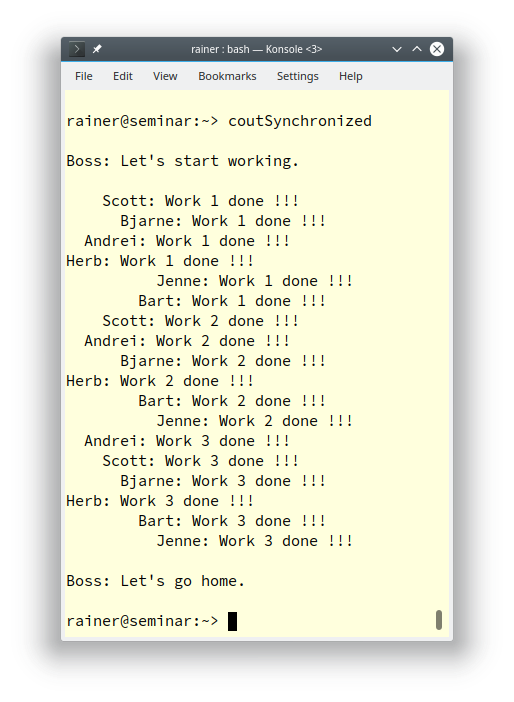
\includegraphics[width=0.8\textwidth]{content/3/chapter6/images/30.png}\\
Synchronized access of std::cout
\end{center}

With C++20, writing synchronized to std::cout is a piece of cake. std::basic\_syncbuf is a wrapper for a \href{https://en.cppreference.com/w/cpp/io/basic_streambuf}{std::basic\_streambuf}. It accumulates output in its buffer. The wrapper sets its content to the wrapped buffer when it is destructed. Consequently, the content appears as a contiguous sequence of characters, and no interleaving of characters can happen.

Thanks to std::basic\_osyncstream, you can directly write synchronously to std::cout.

You can create a named-synchronized output stream. Now, the previous program coutUnsynchronized.cpp is refactored to write synchronized to std::cout.

\hspace*{\fill} \\ %插入空行
\noindent
Synchronized access of std::cout with std::basic\_osyncstream
\begin{lstlisting}[style=styleCXX]
// synchronizedOutput.cpp

#include <chrono>
#include <iostream>
#include <syncstream>
#include <thread>

class Worker{
public:
	Worker(std::string n): name(n) {};
	void operator() (){
		for (int i = 1; i <= 3; ++i) {
			// begin work
			std::this_thread::sleep_for(std::chrono::milliseconds(200));
			// end work
			std::osyncstream syncStream(std::cout);
			syncStream << name << ": " << "Work " << i << " done !!!" << '\n';
		}
	}
private:
std::string name;
};


int main() {

	std::cout << '\n';
	
	std::cout << "Boss: Let's start working.\n\n";
	
	std::thread herb= std::thread(Worker("Herb"));
	std::thread andrei= std::thread(Worker(" Andrei"));
	std::thread scott= std::thread(Worker(" Scott"));
	std::thread bjarne= std::thread(Worker(" Bjarne"));
	std::thread bart= std::thread(Worker(" Bart"));
	std::thread jenne= std::thread(Worker(" Jenne"));
	
	
	herb.join();
	andrei.join();
	scott.join();
	bjarne.join();
	bart.join();
	jenne.join();
	
	std::cout << "\n" << "Boss: Let's go home." << '\n';
	
	std::cout << '\n';

}
\end{lstlisting}

The only change to the previous program coutUnsynchronized.cpp is that std::cout is wrapped in a std::osyncstream (line 16). When the std::osyncstream goes out of scope in line 18, the characters are transferred and std::cout is flushed. It is worth mentioning that the std::cout calls in the main program do not introduce a data race and, therefore, need not be synchronized.

Because I use the syncStream declared on line 17 only once, a temporary object may be more appropriate. The following code snippet presents the modified call operator.


\begin{lstlisting}[style=styleCXX]
void operator()() {
	for (int i = 1; i <= 3; ++i) {
		// begin work
		std::this_thread::sleep_for(std::chrono::milliseconds(200));
		// end work
		std::osyncstream(std::cout) << name << ": " << "Work " << i << " done !!!"
		                            << '\n';
	}
}
\end{lstlisting}

std::basic\_osyncstream syncStream offers two interesting member functions.

\begin{enumerate}
\item 
syncStream.emit() emits all buffered output and executes all pending flushes.

\item 
syncStream.get\_wrapped() returns a pointer to the wrapped buffer.
\end{enumerate}

\href{https://en.cppreference.com/w/cpp/io/basic_osyncstream/get_wrapped}{cppreference.com} shows how you can sequence the output of different output streams with the get\_wrapped member function.

\hspace*{\fill} \\ %插入空行
\noindent
Sequence output
\begin{lstlisting}[style=styleCXX]
// sequenceOutput.cpp

#include <syncstream>
#include <iostream>

int main() {
	
	std::osyncstream bout1(std::cout);
	bout1 << "Hello, ";
	{
		std::osyncstream(bout1.get_wrapped()) << "Goodbye, " << "Planet!" << '\n';
	} // emits the contents of the temporary buffer

	bout1 << "World!" << '\n';
	
} // emits the contents of bout1
\end{lstlisting}

\begin{tcblisting}{breakable,commandshell={}}
Goodbye, Planet!
Hello, World!
\end{tcblisting}

\begin{center}
Synchronized access of std::cout
\end{center}

\begin{tcolorbox}[breakable,enhanced jigsaw,colback=mygreen!5!white,colframe=mygreen!75!black,title={Distilled Information}]
	
\begin{itemize}
\item 
Although std::cout is thread-safe, you may get an interleaving of output operations when threads concurrently write to std::cout. This is only a visual issue but not a data race.

\item 
C++20 supports synchronized output streams. They accumulate output in an internal buffer and write their content in an atomic step. Consequently, no interleaving of output operations happens.
\end{itemize}
	
\end{tcolorbox}



